% Created by tikzDevice version 0.12.6 on 2024-06-11 19:56:27
% !TEX encoding = UTF-8 Unicode
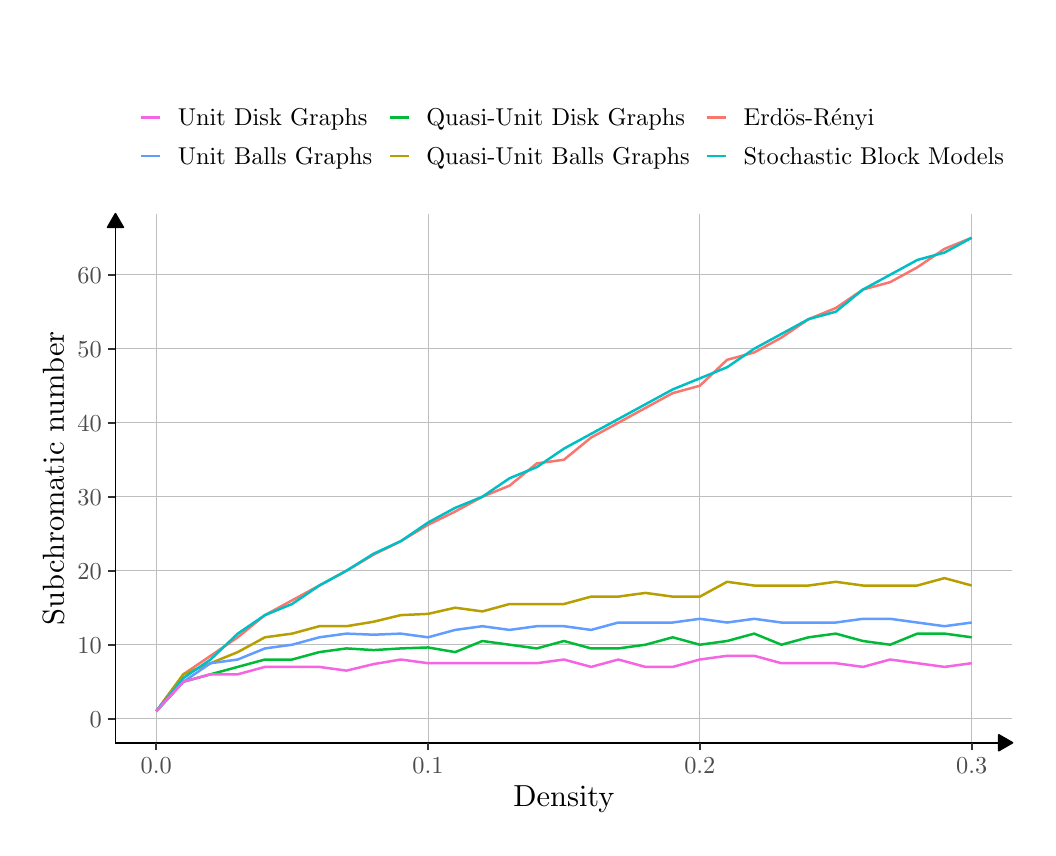
\begin{tikzpicture}[x=1pt,y=1pt]
\definecolor{fillColor}{RGB}{255,255,255}
\path[use as bounding box,fill=fillColor,fill opacity=0.00] (0,0) rectangle (361.35,289.08);
\begin{scope}
\path[clip] (  0.00,  0.00) rectangle (361.35,289.08);
\definecolor{drawColor}{RGB}{255,255,255}
\definecolor{fillColor}{RGB}{255,255,255}

\path[draw=drawColor,line width= 0.6pt,line join=round,line cap=round,fill=fillColor] (  0.00, -0.00) rectangle (361.35,289.08);
\end{scope}
\begin{scope}
\path[clip] ( 31.71, 30.69) rectangle (355.85,221.85);
\definecolor{fillColor}{RGB}{255,255,255}

\path[fill=fillColor] ( 31.71, 30.69) rectangle (355.85,221.85);
\definecolor{drawColor}{RGB}{190,190,190}

\path[draw=drawColor,line width= 0.3pt,line join=round] ( 31.71, 39.38) --
	(355.85, 39.38);

\path[draw=drawColor,line width= 0.3pt,line join=round] ( 31.71, 66.11) --
	(355.85, 66.11);

\path[draw=drawColor,line width= 0.3pt,line join=round] ( 31.71, 92.85) --
	(355.85, 92.85);

\path[draw=drawColor,line width= 0.3pt,line join=round] ( 31.71,119.58) --
	(355.85,119.58);

\path[draw=drawColor,line width= 0.3pt,line join=round] ( 31.71,146.32) --
	(355.85,146.32);

\path[draw=drawColor,line width= 0.3pt,line join=round] ( 31.71,173.06) --
	(355.85,173.06);

\path[draw=drawColor,line width= 0.3pt,line join=round] ( 31.71,199.79) --
	(355.85,199.79);

\path[draw=drawColor,line width= 0.3pt,line join=round] ( 46.45, 30.69) --
	( 46.45,221.85);

\path[draw=drawColor,line width= 0.3pt,line join=round] (144.67, 30.69) --
	(144.67,221.85);

\path[draw=drawColor,line width= 0.3pt,line join=round] (242.89, 30.69) --
	(242.89,221.85);

\path[draw=drawColor,line width= 0.3pt,line join=round] (341.12, 30.69) --
	(341.12,221.85);
\definecolor{drawColor}{RGB}{248,118,109}

\path[draw=drawColor,line width= 0.9pt,line join=round] ( 46.45, 42.05) --
	( 56.27, 55.42) --
	( 66.09, 62.10) --
	( 75.91, 68.79) --
	( 85.74, 76.81) --
	( 95.56, 82.15) --
	(105.38, 87.50) --
	(115.20, 92.85) --
	(125.02, 98.67) --
	(134.85,103.54) --
	(144.67,109.44) --
	(154.49,114.24) --
	(164.31,119.58) --
	(174.14,123.59) --
	(183.96,131.62) --
	(193.78,132.95) --
	(203.60,140.97) --
	(213.43,146.32) --
	(223.25,151.67) --
	(233.07,157.02) --
	(242.89,159.69) --
	(252.72,169.05) --
	(262.54,171.72) --
	(272.36,177.07) --
	(282.18,183.75) --
	(292.00,187.76) --
	(301.83,194.45) --
	(311.65,197.12) --
	(321.47,202.47) --
	(331.29,209.15) --
	(341.12,213.16);
\definecolor{drawColor}{RGB}{183,159,0}

\path[draw=drawColor,line width= 0.9pt,line join=round] ( 46.45, 42.05) --
	( 56.27, 55.42) --
	( 66.09, 59.43) --
	( 75.91, 63.44) --
	( 85.74, 68.79) --
	( 95.56, 70.12) --
	(105.38, 72.80) --
	(115.20, 72.80) --
	(125.02, 74.42) --
	(134.85, 76.81) --
	(144.67, 77.25) --
	(154.49, 79.48) --
	(164.31, 78.14) --
	(174.14, 80.82) --
	(183.96, 80.82) --
	(193.78, 80.82) --
	(203.60, 83.49) --
	(213.43, 83.49) --
	(223.25, 84.83) --
	(233.07, 83.49) --
	(242.89, 83.49) --
	(252.72, 88.84) --
	(262.54, 87.50) --
	(272.36, 87.50) --
	(282.18, 87.50) --
	(292.00, 88.84) --
	(301.83, 87.50) --
	(311.65, 87.50) --
	(321.47, 87.50) --
	(331.29, 90.17) --
	(341.12, 87.50);
\definecolor{drawColor}{RGB}{0,186,56}

\path[draw=drawColor,line width= 0.9pt,line join=round] ( 46.45, 42.05) --
	( 56.27, 52.74) --
	( 66.09, 55.42) --
	( 75.91, 58.09) --
	( 85.74, 60.76) --
	( 95.56, 60.76) --
	(105.38, 63.44) --
	(115.20, 64.77) --
	(125.02, 64.17) --
	(134.85, 64.77) --
	(144.67, 65.12) --
	(154.49, 63.44) --
	(164.31, 67.45) --
	(174.14, 66.11) --
	(183.96, 64.77) --
	(193.78, 67.45) --
	(203.60, 64.77) --
	(213.43, 64.77) --
	(223.25, 66.11) --
	(233.07, 68.79) --
	(242.89, 66.11) --
	(252.72, 67.45) --
	(262.54, 70.12) --
	(272.36, 66.11) --
	(282.18, 68.79) --
	(292.00, 70.12) --
	(301.83, 67.45) --
	(311.65, 66.11) --
	(321.47, 70.12) --
	(331.29, 70.12) --
	(341.12, 68.79);
\definecolor{drawColor}{RGB}{0,191,196}

\path[draw=drawColor,line width= 0.9pt,line join=round] ( 46.45, 42.05) --
	( 56.27, 54.08) --
	( 66.09, 60.76) --
	( 75.91, 70.12) --
	( 85.74, 76.81) --
	( 95.56, 80.82) --
	(105.38, 87.50) --
	(115.20, 92.85) --
	(125.02, 99.01) --
	(134.85,103.54) --
	(144.67,110.25) --
	(154.49,115.57) --
	(164.31,119.58) --
	(174.14,126.27) --
	(183.96,130.28) --
	(193.78,136.96) --
	(203.60,142.31) --
	(213.43,147.66) --
	(223.25,153.00) --
	(233.07,158.35) --
	(242.89,162.36) --
	(252.72,166.37) --
	(262.54,173.06) --
	(272.36,178.40) --
	(282.18,183.75) --
	(292.00,186.43) --
	(301.83,194.45) --
	(311.65,199.79) --
	(321.47,205.14) --
	(331.29,207.81) --
	(341.12,213.16);
\definecolor{drawColor}{RGB}{97,156,255}

\path[draw=drawColor,line width= 0.9pt,line join=round] ( 46.45, 42.05) --
	( 56.27, 52.74) --
	( 66.09, 59.43) --
	( 75.91, 60.76) --
	( 85.74, 64.77) --
	( 95.56, 66.11) --
	(105.38, 68.79) --
	(115.20, 70.12) --
	(125.02, 69.73) --
	(134.85, 70.12) --
	(144.67, 68.79) --
	(154.49, 71.46) --
	(164.31, 72.80) --
	(174.14, 71.46) --
	(183.96, 72.80) --
	(193.78, 72.80) --
	(203.60, 71.46) --
	(213.43, 74.13) --
	(223.25, 74.13) --
	(233.07, 74.13) --
	(242.89, 75.47) --
	(252.72, 74.13) --
	(262.54, 75.47) --
	(272.36, 74.13) --
	(282.18, 74.13) --
	(292.00, 74.13) --
	(301.83, 75.47) --
	(311.65, 75.47) --
	(321.47, 74.13) --
	(331.29, 72.80) --
	(341.12, 74.13);
\definecolor{drawColor}{RGB}{245,100,227}

\path[draw=drawColor,line width= 0.9pt,line join=round] ( 46.45, 42.05) --
	( 56.27, 52.74) --
	( 66.09, 55.42) --
	( 75.91, 55.42) --
	( 85.74, 58.09) --
	( 95.56, 58.09) --
	(105.38, 58.09) --
	(115.20, 56.75) --
	(125.02, 59.11) --
	(134.85, 60.76) --
	(144.67, 59.43) --
	(154.49, 59.43) --
	(164.31, 59.43) --
	(174.14, 59.43) --
	(183.96, 59.43) --
	(193.78, 60.76) --
	(203.60, 58.09) --
	(213.43, 60.76) --
	(223.25, 58.09) --
	(233.07, 58.09) --
	(242.89, 60.76) --
	(252.72, 62.10) --
	(262.54, 62.10) --
	(272.36, 59.43) --
	(282.18, 59.43) --
	(292.00, 59.43) --
	(301.83, 58.09) --
	(311.65, 60.76) --
	(321.47, 59.43) --
	(331.29, 58.09) --
	(341.12, 59.43);
\end{scope}
\begin{scope}
\path[clip] (  0.00,  0.00) rectangle (361.35,289.08);
\definecolor{drawColor}{RGB}{0,0,0}

\path[draw=drawColor,line width= 0.6pt,line join=round] ( 31.71, 30.69) --
	( 31.71,221.85);
\definecolor{fillColor}{RGB}{0,0,0}

\path[draw=drawColor,line width= 0.6pt,line join=round,fill=fillColor] ( 34.56,216.92) --
	( 31.71,221.85) --
	( 28.87,216.92) --
	cycle;
\end{scope}
\begin{scope}
\path[clip] (  0.00,  0.00) rectangle (361.35,289.08);
\definecolor{drawColor}{gray}{0.30}

\node[text=drawColor,anchor=base east,inner sep=0pt, outer sep=0pt, scale=  0.88] at ( 26.76, 36.34) {0};

\node[text=drawColor,anchor=base east,inner sep=0pt, outer sep=0pt, scale=  0.88] at ( 26.76, 63.08) {10};

\node[text=drawColor,anchor=base east,inner sep=0pt, outer sep=0pt, scale=  0.88] at ( 26.76, 89.82) {20};

\node[text=drawColor,anchor=base east,inner sep=0pt, outer sep=0pt, scale=  0.88] at ( 26.76,116.55) {30};

\node[text=drawColor,anchor=base east,inner sep=0pt, outer sep=0pt, scale=  0.88] at ( 26.76,143.29) {40};

\node[text=drawColor,anchor=base east,inner sep=0pt, outer sep=0pt, scale=  0.88] at ( 26.76,170.03) {50};

\node[text=drawColor,anchor=base east,inner sep=0pt, outer sep=0pt, scale=  0.88] at ( 26.76,196.76) {60};
\end{scope}
\begin{scope}
\path[clip] (  0.00,  0.00) rectangle (361.35,289.08);
\definecolor{drawColor}{gray}{0.20}

\path[draw=drawColor,line width= 0.6pt,line join=round] ( 28.96, 39.38) --
	( 31.71, 39.38);

\path[draw=drawColor,line width= 0.6pt,line join=round] ( 28.96, 66.11) --
	( 31.71, 66.11);

\path[draw=drawColor,line width= 0.6pt,line join=round] ( 28.96, 92.85) --
	( 31.71, 92.85);

\path[draw=drawColor,line width= 0.6pt,line join=round] ( 28.96,119.58) --
	( 31.71,119.58);

\path[draw=drawColor,line width= 0.6pt,line join=round] ( 28.96,146.32) --
	( 31.71,146.32);

\path[draw=drawColor,line width= 0.6pt,line join=round] ( 28.96,173.06) --
	( 31.71,173.06);

\path[draw=drawColor,line width= 0.6pt,line join=round] ( 28.96,199.79) --
	( 31.71,199.79);
\end{scope}
\begin{scope}
\path[clip] (  0.00,  0.00) rectangle (361.35,289.08);
\definecolor{drawColor}{RGB}{0,0,0}

\path[draw=drawColor,line width= 0.6pt,line join=round] ( 31.71, 30.69) --
	(355.85, 30.69);
\definecolor{fillColor}{RGB}{0,0,0}

\path[draw=drawColor,line width= 0.6pt,line join=round,fill=fillColor] (350.92, 27.84) --
	(355.85, 30.69) --
	(350.92, 33.53) --
	cycle;
\end{scope}
\begin{scope}
\path[clip] (  0.00,  0.00) rectangle (361.35,289.08);
\definecolor{drawColor}{gray}{0.20}

\path[draw=drawColor,line width= 0.6pt,line join=round] ( 46.45, 27.94) --
	( 46.45, 30.69);

\path[draw=drawColor,line width= 0.6pt,line join=round] (144.67, 27.94) --
	(144.67, 30.69);

\path[draw=drawColor,line width= 0.6pt,line join=round] (242.89, 27.94) --
	(242.89, 30.69);

\path[draw=drawColor,line width= 0.6pt,line join=round] (341.12, 27.94) --
	(341.12, 30.69);
\end{scope}
\begin{scope}
\path[clip] (  0.00,  0.00) rectangle (361.35,289.08);
\definecolor{drawColor}{gray}{0.30}

\node[text=drawColor,anchor=base,inner sep=0pt, outer sep=0pt, scale=  0.88] at ( 46.45, 19.68) {0.0};

\node[text=drawColor,anchor=base,inner sep=0pt, outer sep=0pt, scale=  0.88] at (144.67, 19.68) {0.1};

\node[text=drawColor,anchor=base,inner sep=0pt, outer sep=0pt, scale=  0.88] at (242.89, 19.68) {0.2};

\node[text=drawColor,anchor=base,inner sep=0pt, outer sep=0pt, scale=  0.88] at (341.12, 19.68) {0.3};
\end{scope}
\begin{scope}
\path[clip] (  0.00,  0.00) rectangle (361.35,289.08);
\definecolor{drawColor}{RGB}{0,0,0}

\node[text=drawColor,anchor=base,inner sep=0pt, outer sep=0pt, scale=  1.10] at (193.78,  7.64) {Density};
\end{scope}
\begin{scope}
\path[clip] (  0.00,  0.00) rectangle (361.35,289.08);
\definecolor{drawColor}{RGB}{0,0,0}

\node[text=drawColor,rotate= 90.00,anchor=base,inner sep=0pt, outer sep=0pt, scale=  1.10] at ( 13.08,126.27) {Subchromatic number};
\end{scope}
\begin{scope}
\path[clip] (  0.00,  0.00) rectangle (361.35,289.08);
\definecolor{fillColor}{RGB}{255,255,255}

\path[fill=fillColor] ( 29.26,232.85) rectangle (358.30,266.42);
\end{scope}
\begin{scope}
\path[clip] (  0.00,  0.00) rectangle (361.35,289.08);
\definecolor{fillColor}{RGB}{255,255,255}

\path[fill=fillColor] ( 40.26,252.39) rectangle ( 48.79,260.92);
\end{scope}
\begin{scope}
\path[clip] (  0.00,  0.00) rectangle (361.35,289.08);
\definecolor{drawColor}{RGB}{245,100,227}

\path[draw=drawColor,line width= 0.9pt,line join=round] ( 41.11,256.65) -- ( 47.94,256.65);
\end{scope}
\begin{scope}
\path[clip] (  0.00,  0.00) rectangle (361.35,289.08);
\definecolor{fillColor}{RGB}{255,255,255}

\path[fill=fillColor] ( 40.26,238.35) rectangle ( 48.79,246.89);
\end{scope}
\begin{scope}
\path[clip] (  0.00,  0.00) rectangle (361.35,289.08);
\definecolor{drawColor}{RGB}{97,156,255}

\path[draw=drawColor,line width= 0.9pt,line join=round] ( 41.11,242.62) -- ( 47.94,242.62);
\end{scope}
\begin{scope}
\path[clip] (  0.00,  0.00) rectangle (361.35,289.08);
\definecolor{fillColor}{RGB}{255,255,255}

\path[fill=fillColor] (129.99,252.39) rectangle (138.53,260.92);
\end{scope}
\begin{scope}
\path[clip] (  0.00,  0.00) rectangle (361.35,289.08);
\definecolor{drawColor}{RGB}{0,186,56}

\path[draw=drawColor,line width= 0.9pt,line join=round] (130.85,256.65) -- (137.68,256.65);
\end{scope}
\begin{scope}
\path[clip] (  0.00,  0.00) rectangle (361.35,289.08);
\definecolor{fillColor}{RGB}{255,255,255}

\path[fill=fillColor] (129.99,238.35) rectangle (138.53,246.89);
\end{scope}
\begin{scope}
\path[clip] (  0.00,  0.00) rectangle (361.35,289.08);
\definecolor{drawColor}{RGB}{183,159,0}

\path[draw=drawColor,line width= 0.9pt,line join=round] (130.85,242.62) -- (137.68,242.62);
\end{scope}
\begin{scope}
\path[clip] (  0.00,  0.00) rectangle (361.35,289.08);
\definecolor{fillColor}{RGB}{255,255,255}

\path[fill=fillColor] (244.70,252.39) rectangle (253.24,260.92);
\end{scope}
\begin{scope}
\path[clip] (  0.00,  0.00) rectangle (361.35,289.08);
\definecolor{drawColor}{RGB}{248,118,109}

\path[draw=drawColor,line width= 0.9pt,line join=round] (245.56,256.65) -- (252.39,256.65);
\end{scope}
\begin{scope}
\path[clip] (  0.00,  0.00) rectangle (361.35,289.08);
\definecolor{fillColor}{RGB}{255,255,255}

\path[fill=fillColor] (244.70,238.35) rectangle (253.24,246.89);
\end{scope}
\begin{scope}
\path[clip] (  0.00,  0.00) rectangle (361.35,289.08);
\definecolor{drawColor}{RGB}{0,191,196}

\path[draw=drawColor,line width= 0.9pt,line join=round] (245.56,242.62) -- (252.39,242.62);
\end{scope}
\begin{scope}
\path[clip] (  0.00,  0.00) rectangle (361.35,289.08);
\definecolor{drawColor}{RGB}{0,0,0}

\node[text=drawColor,anchor=base west,inner sep=0pt, outer sep=0pt, scale=  0.88] at ( 54.29,253.62) {Unit Disk Graphs};
\end{scope}
\begin{scope}
\path[clip] (  0.00,  0.00) rectangle (361.35,289.08);
\definecolor{drawColor}{RGB}{0,0,0}

\node[text=drawColor,anchor=base west,inner sep=0pt, outer sep=0pt, scale=  0.88] at ( 54.29,239.59) {Unit Balls Graphs};
\end{scope}
\begin{scope}
\path[clip] (  0.00,  0.00) rectangle (361.35,289.08);
\definecolor{drawColor}{RGB}{0,0,0}

\node[text=drawColor,anchor=base west,inner sep=0pt, outer sep=0pt, scale=  0.88] at (144.03,253.62) {Quasi-Unit Disk Graphs};
\end{scope}
\begin{scope}
\path[clip] (  0.00,  0.00) rectangle (361.35,289.08);
\definecolor{drawColor}{RGB}{0,0,0}

\node[text=drawColor,anchor=base west,inner sep=0pt, outer sep=0pt, scale=  0.88] at (144.03,239.59) {Quasi-Unit Balls Graphs};
\end{scope}
\begin{scope}
\path[clip] (  0.00,  0.00) rectangle (361.35,289.08);
\definecolor{drawColor}{RGB}{0,0,0}

\node[text=drawColor,anchor=base west,inner sep=0pt, outer sep=0pt, scale=  0.88] at (258.74,253.62) {Erdös-Rényi};
\end{scope}
\begin{scope}
\path[clip] (  0.00,  0.00) rectangle (361.35,289.08);
\definecolor{drawColor}{RGB}{0,0,0}

\node[text=drawColor,anchor=base west,inner sep=0pt, outer sep=0pt, scale=  0.88] at (258.74,239.59) {Stochastic Block Models};
\end{scope}
\end{tikzpicture}
